

\begin{figure*}
	\begin{minipage}{\textwidth}
		\begin{minipage}[b]{0.48\textwidth}
			\centering
			\begin{tabular}{llcc}
				\toprule
				Training Set & Model   & Dev set & Test set \\
				\midrule
				\multirow{2}{*}{Train-S} 
				& UCI 				& 23.6 & 23.6\\
				& UCI + RAP 		& 15.9 & 15.9\\
				& UCI + \piecetype 	& 16.1 & 16.2 \\
				\midrule
				\multirow{2}{*}{Train-M} 
				& UCI 				& 11.6 & 11.6\\
				& UCI + RAP 		& 10.4 & 10.4\\
				& UCI + \piecetype 	& 10.1 & 10.0 \\
				\midrule
				\multirow{2}{*}{Train-L} 
				& UCI 				& \phantom{1}7.7 & \phantom{1}7.7\\
				& UCI + RAP 		& \phantom{1}7.4 & \phantom{1}7.4\\
				& UCI + \piecetype 	& \phantom{1}7.2 & \phantom{1}7.2 \\
				\bottomrule
				
			\end{tabular}
			\captionof{table}{Canonical validation and test set perplexity. By canonical we mean that one move, say \pos{f1b5}, counts as one token.}
			\label{tab:perplexity}
		\end{minipage}
		\hfill
		\begin{minipage}[b]{0.48\textwidth}
			\centering
			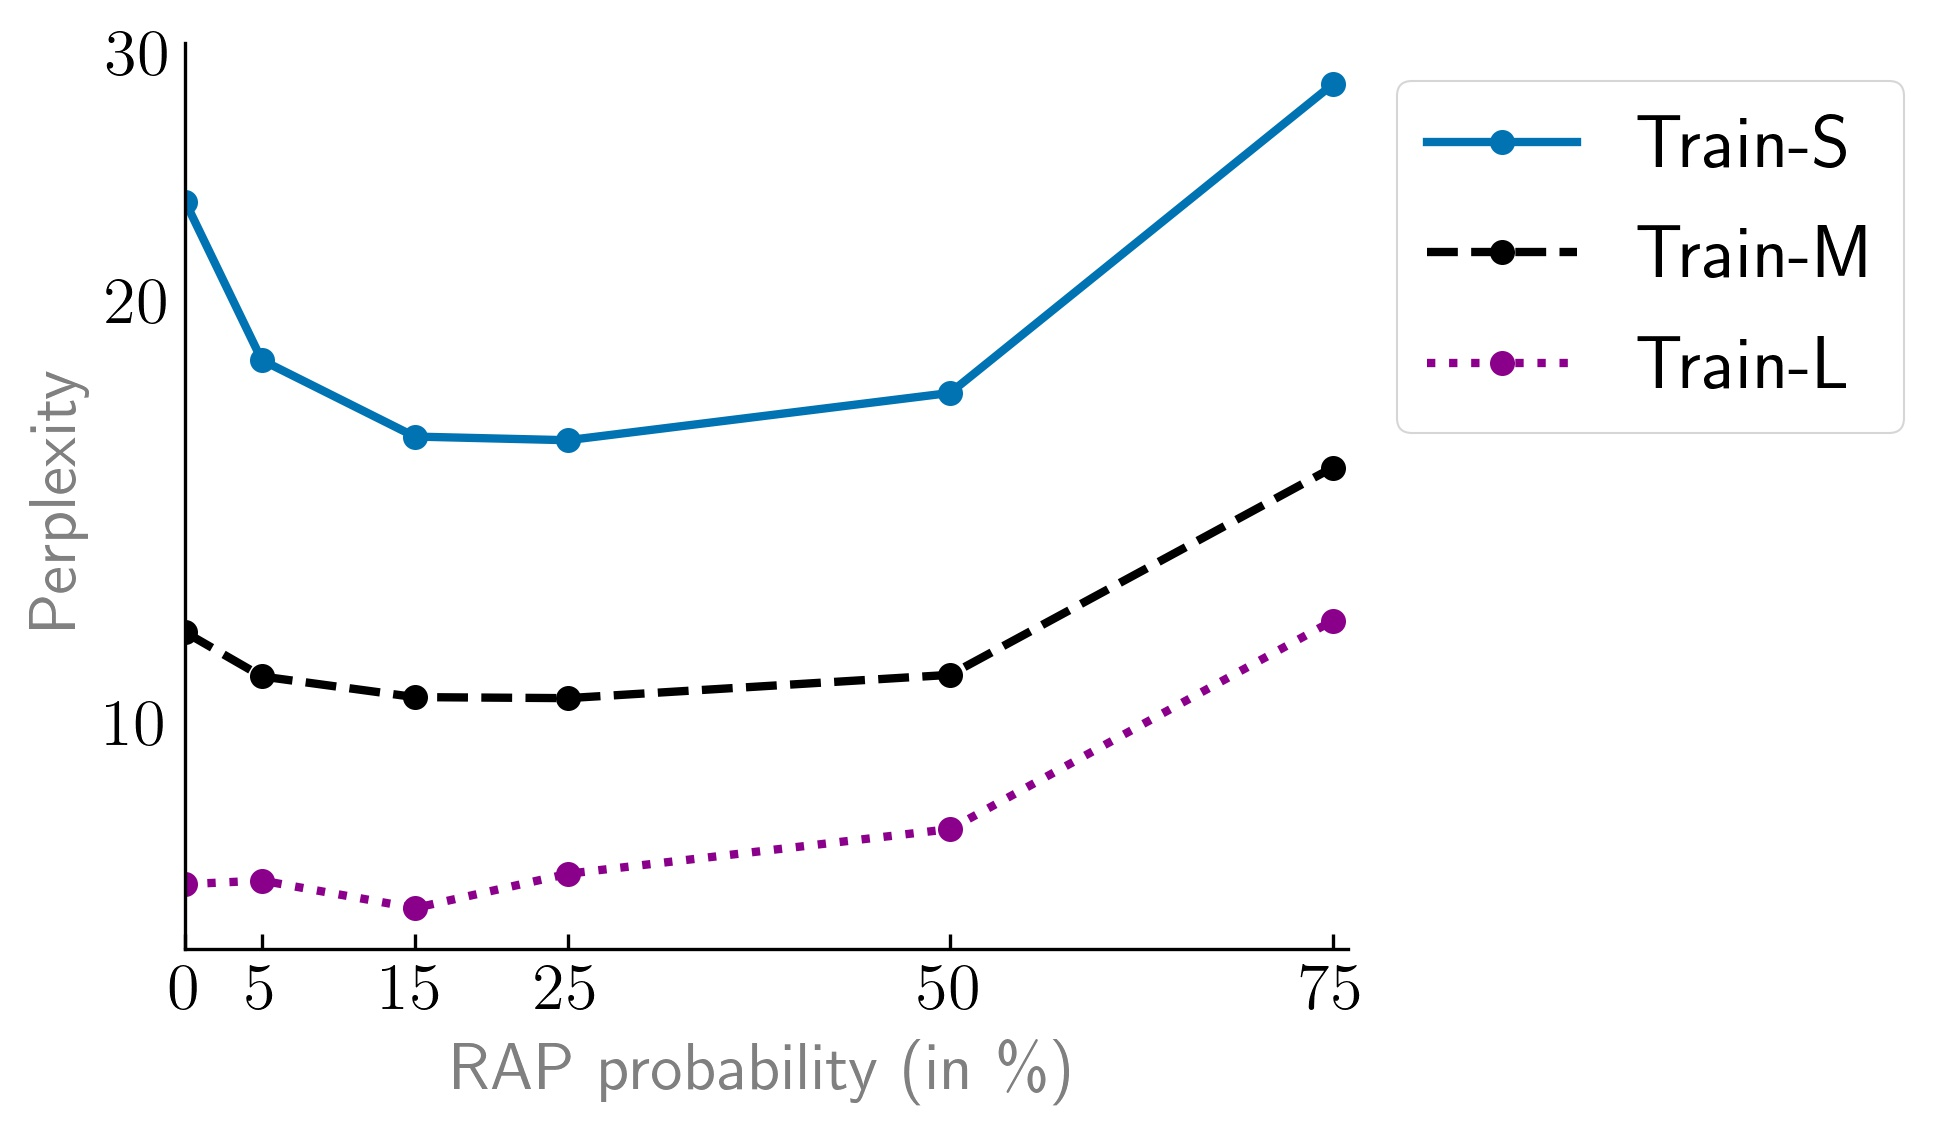
\includegraphics[width=\textwidth]{figures/rap_effect.jpg}
			\captionof{figure}{Validation set perplexities as a function of RAP probabilities for the different training set sizes. RAP $0$ %
				is %
				the standard UCI notation. 
				RAP $100$ is not shown as perplexities are too high. }
			\label{fig:rap_vals}
		\end{minipage}
	\end{minipage}
\end{figure*}